\documentclass[border=10pt]{standalone}

\usepackage{tikz}
\usepackage{tikzsymbols}
\usetikzlibrary{calc,patterns,shapes.geometric}

\def\centerarc[#1](#2)(#3:#4:#5){\draw[#1] ($(#2)+({#5*cos(#3)},{#5*sin(#3)})$) arc (#3:#4:#5);}

\begin{document}
	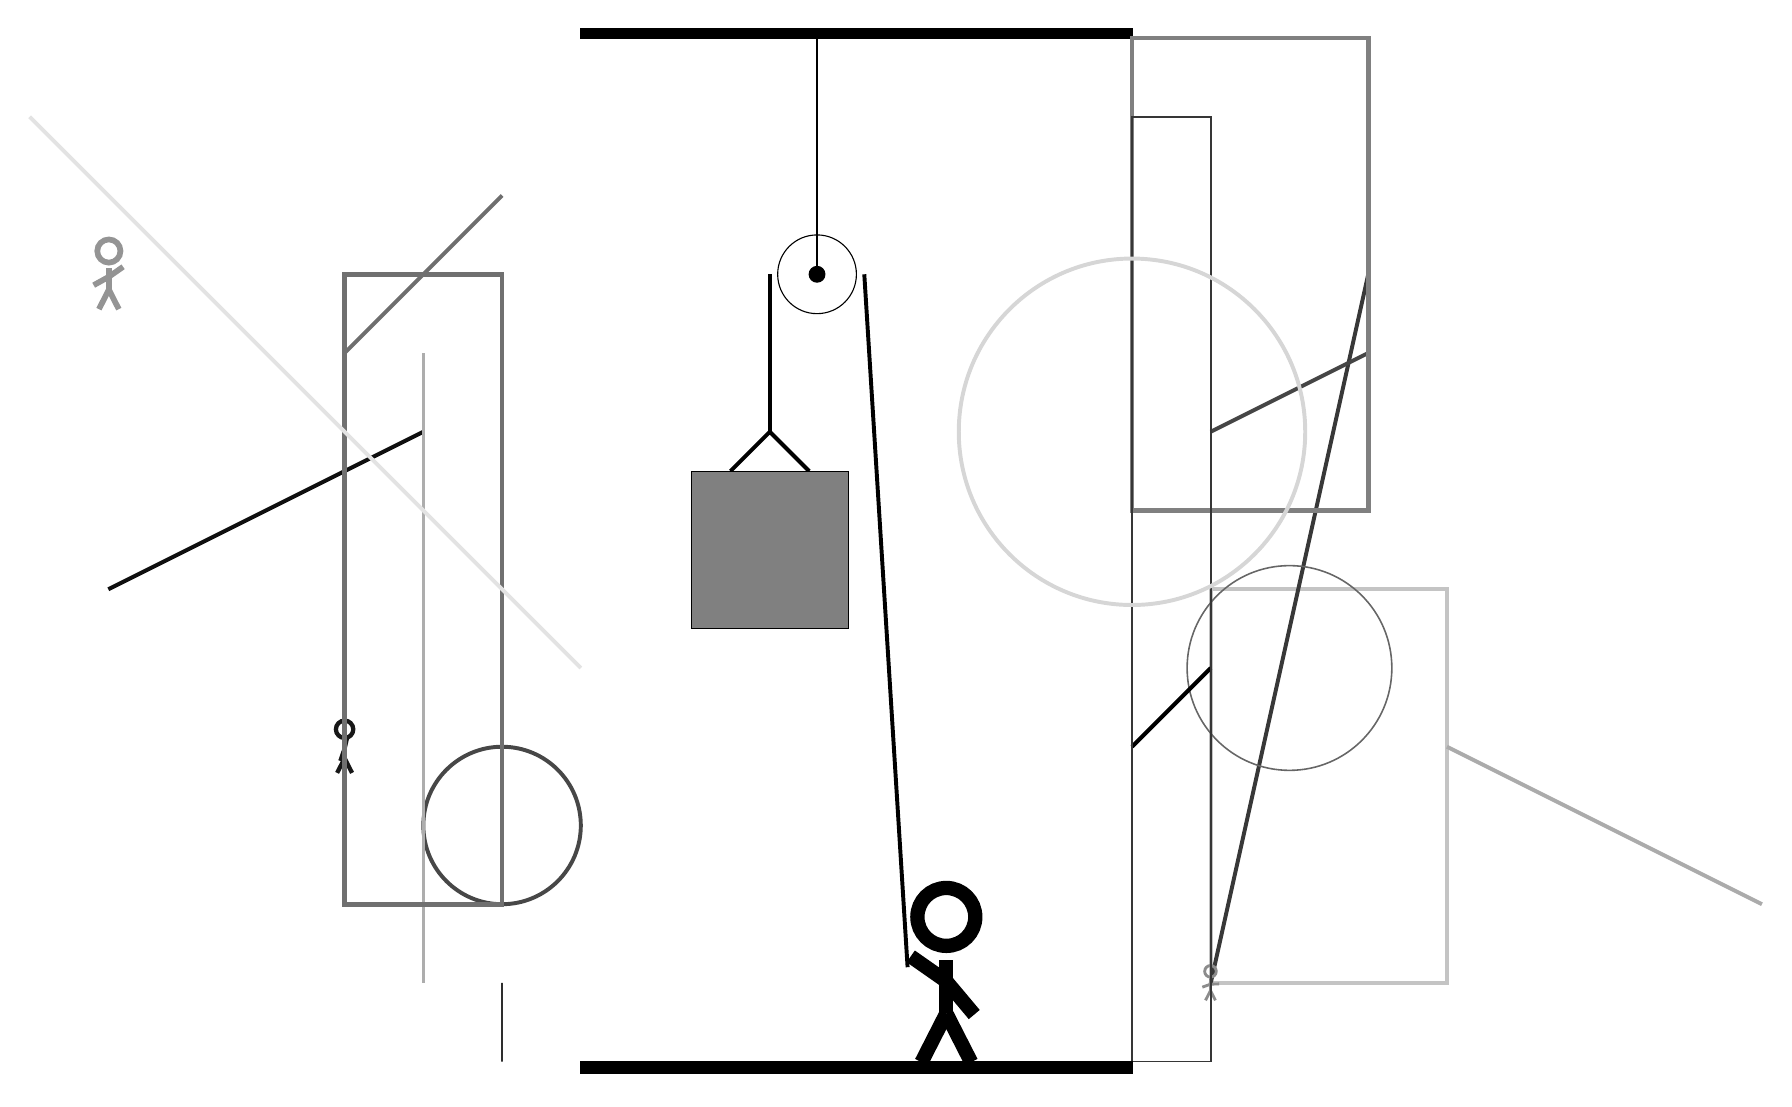
\begin{tikzpicture}
		%%%%% START %%%%%
		
		\draw[fill=black] (-2, 10) rectangle (5, 10.125);
		
		\draw[line width=0.5mm, color=black!23] (6, 3) rectangle (9, -2);
		
		\draw [line width=0.5mm, color=black!72](-3, 0) circle (1.0);
		\draw[line width=0.5mm, color=black!33](9, 1) -- (13, -1);
		\draw[line width=0.5mm, color=black!94](-4, 5) -- (-8, 3);
		
		\draw[line width=0.4mm, color=black!38] (5, 4) rectangle (5, 7);
		
		\draw[line width=0.5mm, color=black!78](8, 7) -- (6, -2);
		\node[line width=0.4mm, color=black!42] at (-8, 7) {\Strichmaxerl[4][29][35]};
		
		\node[line width=0.5mm, color=black!45] at (6, -2) {\Strichmaxerl[2][20][2]};
		\draw [line width=0.2mm, color=black!60](7, 2) circle (1.3);
		
		\draw[line width=0.5mm, color=black!57](-3, 8) -- (-5, 6);
		\draw[line width=0.5mm, color=black!60] (5, 9) rectangle (5, 4);
		\draw[line width=0.4mm, color=black!32] (-4, -2) rectangle (-4, 6);
		\draw[line width=0.5mm, color=black!73](8, 6) -- (6, 5);
		
		\node[line width=0.6mm, color=black!91] at (-5, 1) {\Strichmaxerl[3][71][77]};
		\draw[line width=0.6mm, color=black!56] (-3, -1) rectangle (-5, 7);
		\draw[line width=0.5mm, color=black!11](-2, 2) -- (-9, 9);
		
		\draw[line width=0.6mm, color=black!50] (5, 10) rectangle (8, 4);
		\draw[line width=0.5mm, color=black!100](6, 2) -- (5, 1);
		\draw[line width=0.2mm, color=black!79] (5, -3) rectangle (6, 9);
		\draw[line width=0.3mm, color=black!82] (-3, -3) rectangle (-3, -2);
		\draw [line width=0.5mm, color=black!16](5, 5) circle (2.2);
		
		\draw (1, 7) circle (0.5);
		\draw[fill=black] (1, 7) circle (0.1);
		\draw (1, 10) -- (1, 7);
		
		\draw[line width=0.5mm] (-0.1, 4.5) -- (0.4, 5.0) -- (0.9, 4.5);
		\draw[fill=black!50] (-0.6, 4.5) rectangle (1.4, 2.5);
		
		\draw[line width=0.5mm] (0.4, 7) -- (0.4, 5.0);
		\centerarc[line width=0.5mm](1, 7)(0:180:0.6);
		\draw[line width=0.5mm](1.6, 7) -- (2.15, -1.8);
		
		\node at (2.6, -1.9) {\Strichmaxerl[10][-35][-50]};
		
		\draw[fill=black] (-2, -3) rectangle (5, -3.15);
		
		%%%%% END %%%%%
	\end{tikzpicture}
\end{document}